% Options for packages loaded elsewhere
\PassOptionsToPackage{unicode}{hyperref}
\PassOptionsToPackage{hyphens}{url}
%
\documentclass[
  british,
]{article}
\usepackage{lmodern}
\usepackage{amssymb,amsmath}
\usepackage{ifxetex,ifluatex}
\ifnum 0\ifxetex 1\fi\ifluatex 1\fi=0 % if pdftex
  \usepackage[T1]{fontenc}
  \usepackage[utf8]{inputenc}
  \usepackage{textcomp} % provide euro and other symbols
\else % if luatex or xetex
  \usepackage{unicode-math}
  \defaultfontfeatures{Scale=MatchLowercase}
  \defaultfontfeatures[\rmfamily]{Ligatures=TeX,Scale=1}
\fi
% Use upquote if available, for straight quotes in verbatim environments
\IfFileExists{upquote.sty}{\usepackage{upquote}}{}
\IfFileExists{microtype.sty}{% use microtype if available
  \usepackage[]{microtype}
  \UseMicrotypeSet[protrusion]{basicmath} % disable protrusion for tt fonts
}{}
\makeatletter
\@ifundefined{KOMAClassName}{% if non-KOMA class
  \IfFileExists{parskip.sty}{%
    \usepackage{parskip}
  }{% else
    \setlength{\parindent}{0pt}
    \setlength{\parskip}{6pt plus 2pt minus 1pt}}
}{% if KOMA class
  \KOMAoptions{parskip=half}}
\makeatother
\usepackage{xcolor}
\IfFileExists{xurl.sty}{\usepackage{xurl}}{} % add URL line breaks if available
\IfFileExists{bookmark.sty}{\usepackage{bookmark}}{\usepackage{hyperref}}
\hypersetup{
  pdftitle={Informe VIII},
  pdfauthor={María Alejandra Martínez Guerra},
  pdflang={en-GB},
  hidelinks,
  pdfcreator={LaTeX via pandoc}}
\urlstyle{same} % disable monospaced font for URLs
\usepackage[margin=1in]{geometry}
\usepackage{graphicx,grffile}
\makeatletter
\def\maxwidth{\ifdim\Gin@nat@width>\linewidth\linewidth\else\Gin@nat@width\fi}
\def\maxheight{\ifdim\Gin@nat@height>\textheight\textheight\else\Gin@nat@height\fi}
\makeatother
% Scale images if necessary, so that they will not overflow the page
% margins by default, and it is still possible to overwrite the defaults
% using explicit options in \includegraphics[width, height, ...]{}
\setkeys{Gin}{width=\maxwidth,height=\maxheight,keepaspectratio}
% Set default figure placement to htbp
\makeatletter
\def\fps@figure{htbp}
\makeatother
\setlength{\emergencystretch}{3em} % prevent overfull lines
\providecommand{\tightlist}{%
  \setlength{\itemsep}{0pt}\setlength{\parskip}{0pt}}
\setcounter{secnumdepth}{-\maxdimen} % remove section numbering
\usepackage{pgf,tikz}
\ifxetex
  % Load polyglossia as late as possible: uses bidi with RTL langages (e.g. Hebrew, Arabic)
  \usepackage{polyglossia}
  \setmainlanguage[variant=british]{english}
\else
  \usepackage[shorthands=off,main=british]{babel}
\fi

\title{Informe VIII}
\usepackage{etoolbox}
\makeatletter
\providecommand{\subtitle}[1]{% add subtitle to \maketitle
  \apptocmd{\@title}{\par {\large #1 \par}}{}{}
}
\makeatother
\subtitle{Econometric Modeling and Solving Social Problems}
\author{María Alejandra Martínez Guerra}
\date{14 julio 2020}

\begin{document}
\maketitle

\hypertarget{introducciuxf3n}{%
\section{Introducción}\label{introducciuxf3n}}

En el presente informe VIII del seminario EII del doctorado en
Ingeniería Industrial de la Pontificia Universidad Católica de
Valparaíso se analizaran 3 trabajos de investigación relacionados con
modelos econométricos, como a través de ellos y del uso de sus
herramientas estos modelos permiten resolver problemas sociales, es
decir Fuente-Mella et al. (2020) analiza que por medio del uso de las
herramientas econométricas cuantitativas se puede dar solución a algunos
problemas de la vida real. Mejorando considerablemente la calidad de
vida de las personas en una comunidad, ya sea respecto al manejo de los
recursos, seguridad vial y toma de decisiones en las crisis económicas
financieras.

\hypertarget{anuxe1lisis-de-la-literatura-relacionada}{%
\section{Análisis de la literatura
Relacionada}\label{anuxe1lisis-de-la-literatura-relacionada}}

De los 80 en adelante se empezó a estudiar seriamente problemáticas
asociados a estas investigaciones. Los modelos econométricos son
posiblemente la especificación económica más determinada para analizar
el efecto o impacto de un cambio sobre un sistema social. Fuente-Mella
et al. (2020)

Mediante la revisión de literatura con palabras claves como
\emph{Econometric Modeling}, \emph{Modelos de Series T emporales} y
\emph{Modelos de Cortes T rasversales} se encontró una diversidad de
planteamientos y consideraciones en este tipo de investigaciones por
parte de (Hanns de la Fuente) y otros autores en otros países, así como
su aplicación en distintas áreas. La plataforma científica que se
utilizo fue web of science dando como resultado mas de 400 papers
relacionados y publicaciones en revistas; de los cuales 175 son de EEUU,
18 c son investigaciones provenientes de china, etc.

\includegraphics[width=0.5\linewidth]{Informe-de-la-fuente_files/figure-latex/unnamed-chunk-2-1}
\includegraphics[width=0.5\linewidth]{Informe-de-la-fuente_files/figure-latex/unnamed-chunk-2-2}
\includegraphics[width=0.5\linewidth]{Informe-de-la-fuente_files/figure-latex/unnamed-chunk-2-3}
\includegraphics[width=0.5\linewidth]{Informe-de-la-fuente_files/figure-latex/unnamed-chunk-2-4}
\includegraphics[width=0.5\linewidth]{Informe-de-la-fuente_files/figure-latex/unnamed-chunk-2-5}

\includegraphics{Informe-de-la-fuente_files/figure-latex/unnamed-chunk-3-1.pdf}

Una gran parte de las áreas temáticas en las que están enfocadas estas
investigaciones para mencionar solo algunas son: Ciencias Sociales
Aplicadas con 126 publicaciones, Humanidades con 17, Ingenieríıas con
16, Ciencias Agrícolas con 9, Ciencias de la Salud 6, Ciencias
Biológicas y Ciencias Exactas y de la Tierra con 4 publicaciones
respectivamente. También en dicha plataforma se lograron visualizar que
los idiomas en los que prevalece este tipo de investigación son en
Español, Inglés y Portugués. En los graficos notamos que el estudio en
esta area ha sido bastante oscilate pero se observa un crecimiento a lo
largo de los años ha sido notorio en este ramo, note que la importancia
que tiene para el mundo actualmente investigaciones relacionadas con las
palabras clave. Pero en 2019 pese a que aún tiene un grado alto de
publicaciones importantes en 2020 decae precipitadamente.

\hypertarget{marco-teuxf3rico-descripciuxf3n-general}{%
\section{Marco Teórico (Descripción
General)}\label{marco-teuxf3rico-descripciuxf3n-general}}

\hypertarget{planteamiento-del-problema}{%
\subsection{Planteamiento del
Problema}\label{planteamiento-del-problema}}

En Chile, los ayuntamientos son fundamentales para la descentralización
del país, puesto que representa un camino para estar más conectado con
las personas, sus problemas, necesidades y deseos. Por lo anterior, los
elementos que lo hacen eficiente y mejoran la calidad de vida de los
ciudadanos son esenciales. Hay 346 ayuntamientos en Chile que pertenecen
a las diferentes comunas, pero para la investigación se seleccionaron
los que tienen más de 50,000 habitantes y que pertenecen a las capitales
regionales con características diferentes.

De la presente investigación nos centraremos principalmente en como a
partir de estos modelos se pueden llegar a medir, cuantificar muchos
problemas de tipo social y real llegando inclusive a poder predecir al
final de las investigaciones.

\begin{itemize}
\tightlist
\item
  \textbf{En el caso 1 (Analysis of the Factors of Chilean City Hall
  Using Econometric Modeling and Stochastic Frontier)}, se desarrolló un
  modelo econométrico que explicaba los factores determinados para la
  eficiencia del ayuntamiento en Chile, es decir, se diseñó un modelo
  que es capaz de determinar los factores que influyen en la eficiencia
  del ayuntamiento en función del índice de calidad de vida de las
  ciudades (bajo ciertas circunstancias) y muestra los aspectos que
  requieren atención especial en las nuevas políticas públicas sobre la
  gestión del Ayuntamiento. Se utilizaron modelos de regresión, paso a
  paso, ClusterDendogram jerárquico y cluster k-means para conocer por
  medio del análisis de eficiencia cuales eran las variables que
  permitirían mejorar la calidad de vida dentro de las municipalidades.
  Los datos con los que se trabajó en la investigación fueron tomados de
  \url{http://datos.gob.cl/https://reportescomunales.bcn.cl/}, en la
  Figura 1, se observa los 6 modelos de regresión ajustado.
\end{itemize}

\begin{figure}[htbp]
\centering
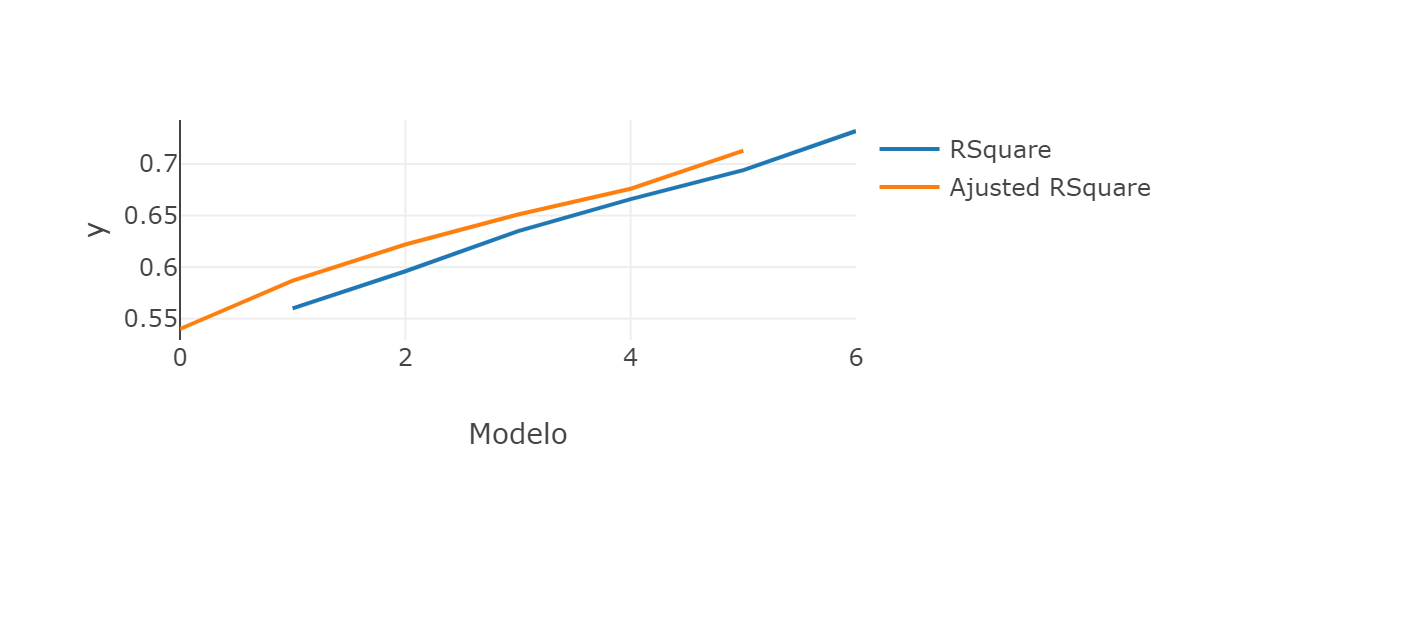
\includegraphics{caso1}
\caption{Regression Models-Stepwise}
\end{figure}

\begin{itemize}
\tightlist
\item
  \textbf{En el caso 2 Forecasting Performance Measures for Traffic
  Safety using Deterministic and Stochastic Models} en 2012 Barack Obama
  aprobó la ley \emph{(Map-21)}, \url{https://www.fhwa.dot.gov/map21/}
  donde se destinaron elevados recursos en millones de dólares para el
  estudio de todo el sistema de trasporte de Estados Unidos, en donde se
  tenían que tener en cuenta ciertos aspectos que se debían modelar como
  mejoramiento de seguridad vial, trafico etc. Paz et al. (2015) Los
  datos utilizados de 2001 a 2014 fueron anualmente e igualmente
  espaciados. Las variables que se tuvieron en cuenta son:
\item
  La cantidad de muertes -La cantidad de lesiones graves
\item
  Muertes por vehículo Millas recorridas (VMT)
\item
  Lesiones graves por VMT
\end{itemize}

El problema que se debía modelar es \textbf{¿Qué metodología utilizar,
según los DOT estatales, para pronosticar medidas de desempeño de
seguridad a fin de establecer objetivos para la reducción de muertes y
lesiones graves y alcanzar los objetivos de la política MAP-21?}

Con el objetivo de facilitar la gestión financiera y la toma de
decisiones asociadas a el problema anterior se utilizaron métodos de
pronóstico deterministas como Simple, Holt, Brown y Damped Trend, y el
pronóstico estocástico utilizó \(ARIMA(p, d, q)\).

Este modelo \(ARIMA(p, d, q)\), viene daro por:

\begin{eqnarray}
\hat{y}_{t}=\phi_{0}+\sum_{i=1}^{p}\phi_\phi_{i}y_{t-1}-\sum_{i=1}^{q}\theta_{i}\epsilon_{t-1}+\epsilon_{t}
\end{eqnarray}

Donde

\begin{eqnarray*}
    y_{t}=Y_{t} \mbox{for d=0}\\
    y_{t}= Y_{t}-Y_{t-1}\mbox{for d=1}\\
    y_{t}= Y_{t}-(Y_{t-1})-(Y_{t-2})\mbox{for d=1}\\    
\end{eqnarray*}

\begin{itemize}
\tightlist
\item
  \textbf{En el caso 3 Gobiernos Corporativos y Asimetrías de
  Información. Modelamiento Econométrico del Spread ( Bid Ask) para una
  muestra de Empresas Chilenas.} De este caso se destaca para mayor
  comprensión del lector la medida de asimetría de información, que se
  presenta cuando los mercados de capitales, proporcionan una relación
  significativa entre la oferta y el grado de divulgación dada por las
  empresas al mercado de capitales. Para llevar a cabo el estudio se
  utiliza un análisis empírico de una empresa chilena que representa el
  38\% de la capitalización de mercado total de la IPSA. Los resultados
  proporcionan que solo los factores, la cantidad ofrecida y el corredor
  involucrado en él, son relevantes para explicar la oferta-demanda
  (spread). Heckman and Vytlacil (2007)
\end{itemize}

\hypertarget{contribuciuxf3n-del-trabajo}{%
\subsection{Contribución del
Trabajo}\label{contribuciuxf3n-del-trabajo}}

Existen muchos problemas asociados a fenómenos de la vía real que se
pueden solucionar utilizando modelos econométricos y ciertas
herramientas de tipo matemático. Además de esto la primera investigación
nos permite contrastar entre diferentes ayuntamientos (Norte, Centro y
Sur) para así conocer los factores que determinan y afectan la
eficiencia de las municipalidades de acuerdo al uso de los recursos (lo
que finalmente afecta tanto de manera positiva como negativa la calidad
de vida de las personas). Para el segundo caso Fuente-Mella et al.
(2013) que va como hacia la misma línea de investigación, se evidencia
como resultado que los métodos Simple y Holt proporcionaron un
pronóstico adecuado para el 28\% de los casos. Marrón este método
proporcionó un pronóstico adecuado para el 44\% de los casos. Sin
embargo, el proceso estocástico, el método ARIMA, no encontró una bondad
de ajuste aceptable. Pero es algo que se puede mejorar si se decide
modelar grandes conjuntos de datos. Este estudio no se había realizado
antes ya que comprende todo el sistema complejo de un país y se intenta
modelar ciertos aspectos solo con 4 variables determinadas como las de
interés para el objetivo final de la investigación.

\tikzset{every picture/.style={line width=0.75pt}} \%set default line
width to 0.75pt

\begin{tikzpicture}[x=0.75pt,y=0.75pt,yscale=-1,xscale=1]
%uncomment if require: \path (0,310); %set diagram left start at 0, and has height of 310

%Shape: Axis 2D [id:dp046885868423533594] 
\draw  (102,197) -- (357.61,197)(127.56,25) -- (127.56,216.11) (350.61,192) -- (357.61,197) -- (350.61,202) (122.56,32) -- (127.56,25) -- (132.56,32)  ;
%Straight Lines [id:da46666184664814647] 
\draw [color={rgb, 255:red, 208; green, 2; blue, 27 }  ,draw opacity=1 ]   (128,66) -- (290.61,66.11) -- (301.61,66.11) ;
%Straight Lines [id:da14926473657081063] 
\draw    (126,112) -- (253.61,110.11) ;
%Straight Lines [id:da437990954245274] 
\draw [color={rgb, 255:red, 126; green, 211; blue, 33 }  ,draw opacity=1 ]   (127,158) -- (300.61,158.11) ;
%Shape: Brace [id:dp7115646828204212] 
\draw   (311.61,148.11) .. controls (316.28,148.18) and (318.64,145.88) .. (318.71,141.21) -- (318.97,122.21) .. controls (319.06,115.54) and (321.44,112.24) .. (326.11,112.31) .. controls (321.44,112.24) and (319.16,108.88) .. (319.25,102.21)(319.21,105.21) -- (319.52,83.21) .. controls (319.59,78.54) and (317.29,76.18) .. (312.62,76.11) ;
%Straight Lines [id:da49507300460925485] 
\draw    (317.61,175.11) -- (177.61,41.11) ;
%Straight Lines [id:da8837001984090413] 
\draw    (317.61,50.11) -- (173.11,183.61) ;

% Text Node
\draw (61,61) node [anchor=north west][inner sep=0.75pt]  [font=\footnotesize,color={rgb, 255:red, 208; green, 2; blue, 27 }  ,opacity=1 ] [align=left] {precio ask};
% Text Node
\draw (70,95) node [anchor=north west][inner sep=0.75pt]  [font=\footnotesize,color={rgb, 255:red, 208; green, 2; blue, 27 }  ,opacity=1 ] [align=left] {\textcolor[rgb]{0,0,0}{{\small precio}}\\\textcolor[rgb]{0,0,0}{{\small equilibrio}}};
% Text Node
\draw (64,148) node [anchor=north west][inner sep=0.75pt]  [color={rgb, 255:red, 208; green, 2; blue, 27 }  ,opacity=1 ] [align=left] {\textcolor[rgb]{0.49,0.83,0.13}{{\footnotesize precio bid}}};
% Text Node
\draw (213,47) node [anchor=north west][inner sep=0.75pt]  [color={rgb, 255:red, 208; green, 2; blue, 27 }  ,opacity=1 ] [align=left] {{\scriptsize Orden compra}};
% Text Node
\draw (219,141) node [anchor=north west][inner sep=0.75pt]  [color={rgb, 255:red, 208; green, 2; blue, 27 }  ,opacity=1 ] [align=left] {\textcolor[rgb]{0,0,0}{{\scriptsize Orden venta}}};
% Text Node
\draw (331,106) node [anchor=north west][inner sep=0.75pt]  [font=\footnotesize,color={rgb, 255:red, 208; green, 2; blue, 27 }  ,opacity=1 ] [align=left] {\textcolor[rgb]{0,0,0}{spread (bid-ask)}};
% Text Node
\draw (317,38) node [anchor=north west][inner sep=0.75pt]  [color={rgb, 255:red, 0; green, 0; blue, 0 }  ,opacity=1 ] [align=left] {S};
% Text Node
\draw (324,170) node [anchor=north west][inner sep=0.75pt]  [color={rgb, 255:red, 208; green, 2; blue, 27 }  ,opacity=1 ] [align=left] {\textcolor[rgb]{0,0,0}{D}};


\end{tikzpicture}

\hypertarget{comentario-adicional}{%
\subsection{Comentario Adicional}\label{comentario-adicional}}

Se podría incluir en un nuevo trabajo como extensión del caso 2 nuevas
variables y determinar si influyen de manera significativa en el modelo
o si definitivamente el modelo debe tener solo 4 variables de decisión.
También a través de la misma línea de investigación y de estos modelos
estudiar el impacto que puede generar un cambio en la forma como se
utilizan y se aprovechan los recursos de las municipalidades. Luego
después de esto analizar si hay un cambio en el manejo de las políticas
públicas que tipo de efecto causa en el sistema.

\hypertarget{references}{%
\section*{References}\label{references}}
\addcontentsline{toc}{section}{References}

\hypertarget{refs}{}
\leavevmode\hypertarget{ref-fuente-mella_econometric_2013}{}%
Fuente-Mella, H. de la, Campos-Espinoza, R., Silva-Palavecinos, B.,
Cademartori-Rosso, D., 2013. An Econometric Analysis for the Behavior of
the Bid-Ask Spread. Open Journal of Social Sciences 1, 1--5.
\url{https://doi.org/10.4236/jss.2013.17001}

\leavevmode\hypertarget{ref-de_la_fuente-mella_econometric_2020}{}%
Fuente-Mella, H. de la, Rojas Fuentes, J.L., Leiva, V., 2020.
Econometric modeling of productivity and technical efficiency in the
Chilean manufacturing industry. Computers \& Industrial Engineering 139,
105793. \url{https://doi.org/10.1016/j.cie.2019.04.006}

\leavevmode\hypertarget{ref-heckman_chapter_2007}{}%
Heckman, J.J., Vytlacil, E.J., 2007. Chapter 70 Econometric Evaluation
of Social Programs, Part I: Causal Models, Structural Models and
Econometric Policy Evaluation, in: Heckman, J.J., Leamer, E.E. (Eds.),
Handbook of Econometrics. Elsevier, pp. 4779--4874.
\url{https://doi.org/10.1016/S1573-4412(07)06070-9}

\leavevmode\hypertarget{ref-paz_forecasting_2015}{}%
Paz, A., Veeramisti, N., de la Fuente-Mella, H., 2015. Forecasting
performance measures for traffic safety using deterministic and
stochastic models, in: 2015 IEEE 18th International Conference on
Intelligent Transportation Systems. pp. 2965--2970.
\url{https://doi.org/10.1109/ITSC.2015.475}

\end{document}
